% ju 01-Dec-24 mein-dokument.tex
\documentclass{content/vorlage-design-main}
% Verwenden von fontspec und unicode-math für XeLaTeX oder LuaLaTeX

%% Ganze Überschrift
\title{Anwendung von Markdown-Techniken für Dokumentationen}
%% Kürzerer Titel
\runningtitle{Dokumentation mit Markdown}
\author{Jan Unger}
\date{\today}

%% Referenzen
\addbibresource{content/literatur.bib}

\begin{document}

\maketitle

\begin{abstract}
Markdown Ein 2004 von Gruber/Swartz entwickeltes leichtgewichtiges
Auszeichnungsformat für menschen- und maschinenlesbare formatierte
Texte. Ideal für technische Dokumentation.

Pandoc Ein von MacFarlane entwickelter universeller Dokumentenkonverter
für verschiedene Markup-Formate. Open-Source-Tool für akademische und
technische Dokumentation.

LaTeX Ein 1984 von Lamport entwickeltes Textsatzsystem (basierend auf
Knuths TeX, 1978). Standard für wissenschaftliche Publikationen mit
hochwertiger Typografie und Formelsatz.

Python Eine 1991 von van Rossum entwickelte Programmiersprache mit
klarer Syntax. Anwendung in Wissenschaft, Datenanalyse, KI und
Webentwicklung.

Git Ein 2005 von Torvalds entwickeltes verteiltes
Versionskontrollsystem. Standard für Softwareprojekte mit Branch-Konzept
für parallele Entwicklung.

\textbf{Keywords:} Markdown, Pandoc, Latex, Python, Git
\end{abstract}

\subsection{Git}\label{git}

\begin{figure}
\centering
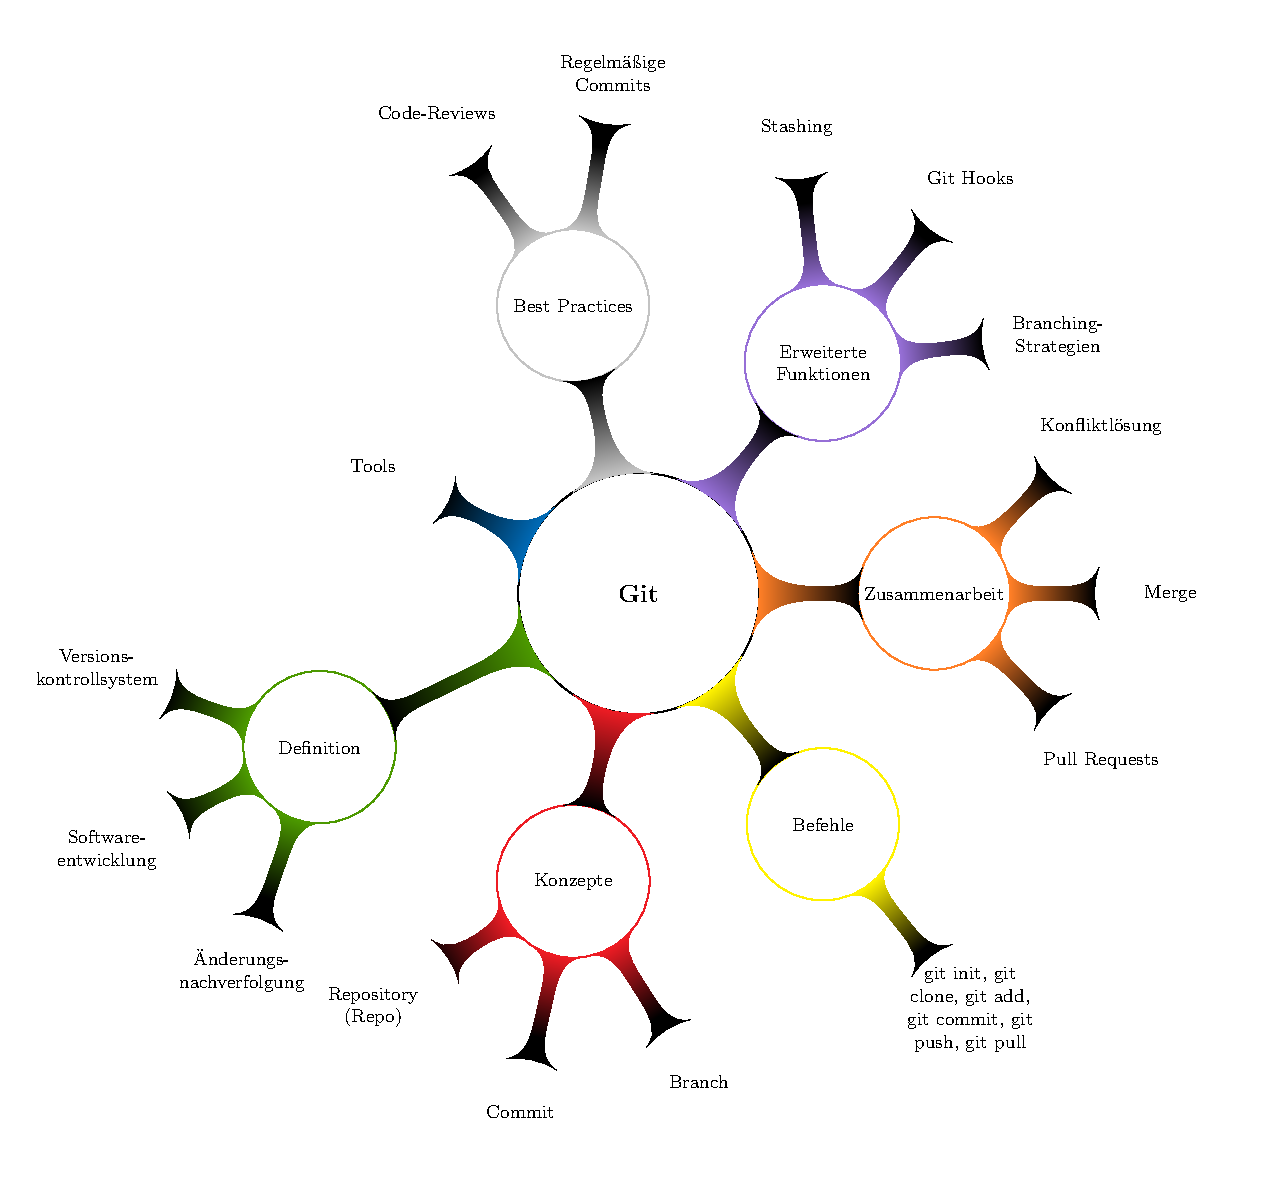
\includegraphics[width=0.6\linewidth,keepaspectratio]{images/Mindmap-Git.pdf}
%\floatnotes{}
%\label{fig:}
\caption{Was ist Git?}
\end{figure}

\begin{lstlisting}[language=bash]
# GitHub-Anmeldung und Zugangsdaten zwischenspeichern
gh auth login
git config --global credential.helper cache

# Remote-Verbindungen anzeigen
git remote -v

# Lokales Backup-Repository einrichten
git init --bare
git remote add local /Users/jan/notizen_latex_html_python_v1.3.git
git remote rename localBackup local
git push local main
git pull local main

# GitHub-Repository einrichten
git init
git remote add origin git@github.com:ju1-eu/notizen_latex_html_python_v1.3.git
git branch -M main
git push -u origin main
git pull origin main

# Standardbefehle für Synchronisation
git push  # Änderungen hochladen
git pull  # Änderungen herunterladen
git st    # Status anzeigen
git ls    # Dateien auflisten

# Repository klonen
git clone https://github.com/ju1-eu/notizen_latex_html_python_v1.3.git
git clone /Users/jan/notizen_latex_html_python_v1.3.git notizen_klon
\end{lstlisting}

\subsection{Latex}\label{latex}

\begin{lstlisting}[language=bash]
# TeX Live Manager und Updates
wget https://mirror.ctan.org/systems/texlive/tlnet/update-tlmgr-latest.sh # Manager herunterladen
sudo sh update-tlmgr-latest.sh -- --accept # Update ausführen
sudo chown -R $(whoami) /usr/local/texlive/ # Nutzerrechte setzen

# Paket-Management
tlmgr install pgf # PGF/TikZ-Paket installieren
tlmgr update --all # Alle Pakete aktualisieren

# System-Überprüfung
tlmgr --version # Version anzeigen
tlmgr list --installed # Installierte Pakete auflisten
\end{lstlisting}

\section{Markdown}\label{markdown}

\subsection{Quellenangabe}\label{quellenangabe}

\begin{itemize}

\item
  Fachbuchautor \textcite{dalwigk:2024:fachbuchautor}.
\item
  Online Kurse \textcite{schaffranek:2024:kurse}.
\item
  Hacking und Cyber Security mit KI \textcite{dalwigk:2023:hacking}.
\item
  Python für Einsteiger \textcite{dalwigk:2022:python}.
\item
  Mikrocontroller ESP32 \textcite{brandes:2023:mikrocontroller}.
\item
  Roboterauto \textcite{brandes:2022:esp32}.
\item
  Daten mit Raspberry Pi im Netz speichern und visualisieren
  \textcite{brandes:2023:daten}.
\end{itemize}

Hier ist ein Text, der eine Fußnote benötigt.\footnote{Text der Fußnote.}

\subsection{Liste}\label{liste}

\begin{enumerate}
\def\labelenumi{\arabic{enumi}.}

\item
  eins
\item
  zwei
\end{enumerate}

\begin{itemize}

\item
  neu
\item[$\square$]
  check
\item[$\boxtimes$]
  gecheckt
\end{itemize}

\subsection{Tabelle}\label{tabelle}

\textbf{Tabelle 1:} Diese Tabelle gibt eine übersichtliche Darstellung
der ausgeführten Skripte, ihrer jeweiligen Funktionen.

\begin{table}[ht]
  %\caption{}
  %\label{tab:my-table}
  \begin{tabular}{@{}ll@{}}
\toprule
Skriptname
 &
Beschreibung
 \\
\midrule[\heavyrulewidth]
\verb|html1\_konverter\_pandoc.py| & Konvertiert
HTML-Dokumente mit Pandoc \\
\verb|html2\_dateien\_verarbeiten.py| & Verarbeitet
HTML-Dateien \\
\verb|html3\_navigation.py| & Erzeugt
Navigationsseiten \\
\verb|html4\_entfernen.py| & Entfernt HTML-Markup \\
\verb|latex\_convert1.py| & Konvertiert
LaTeX-Dokumente \\
\verb|latexcode\_entfernen2.py| & Entfernt
LaTeX-Markup \\
\verb|dokumentation.py| & Erstellt
Projekt-Dokumentation \\
\verb|dateien\_inhaltsverzeichnis.py| & Generiert
Datei-Index \\
\verb|git\_hilfsprogramm.py| & Git-Hilfsfunktionen \\
\verb|scriptauswahl.py| & Skript-Auswahlmenü \\
\verb|suchen\_ersetzen.py| & Text suchen/ersetzen \\
\verb|sync\_tex.py| & Synchronisiert TeX-Dateien \\
\verb|image\_resizer.py| & Bildgrößen anpassen \\
\verb|create\_gallery.py| & Erstellt Bildergalerie \\
\verb|extract\_pdf\_images.py| & Extrahiert Bilder
aus PDFs \\
\verb|pdf\_extractor.py| & PDF-Daten extrahieren \\
\verb|youtube\_text\_extraktor.py| &
YouTube-Untertitel extrahieren \\
\bottomrule
\end{tabular}%
\end{table}

\subsection{Bilder}\label{bilder}

\begin{figure}
\centering

\includegraphics[width=0.4\linewidth,keepaspectratio]{images/Logo/Logo2.pdf}
%\floatnotes{}
%\label{fig:}
\caption{Logo 2}
\end{figure}

\begin{figure}
\centering
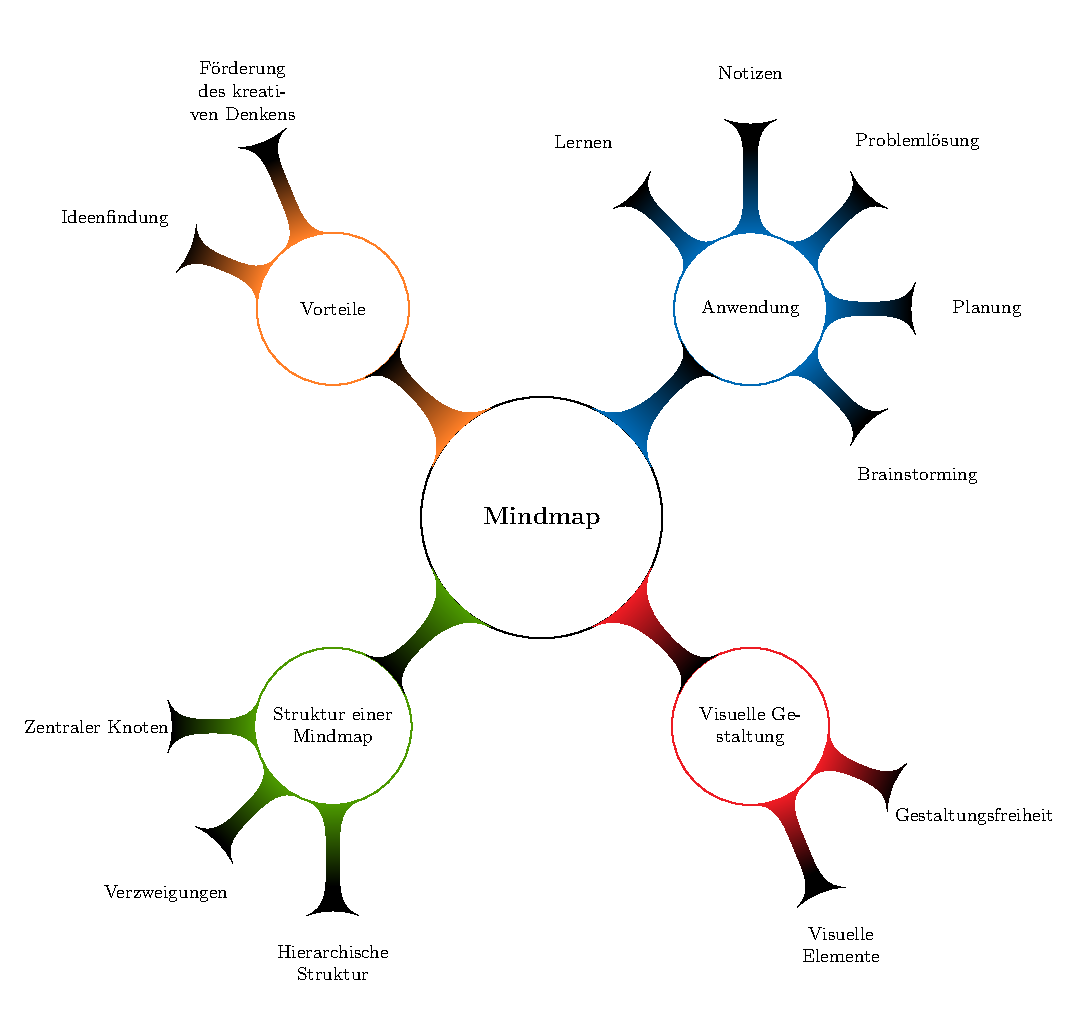
\includegraphics[width=0.6\linewidth,keepaspectratio]{images/Mindmap.pdf}
%\floatnotes{}
%\label{fig:}
\caption{Was ist eine Mindmap?}
\end{figure}

\begin{figure}
\centering
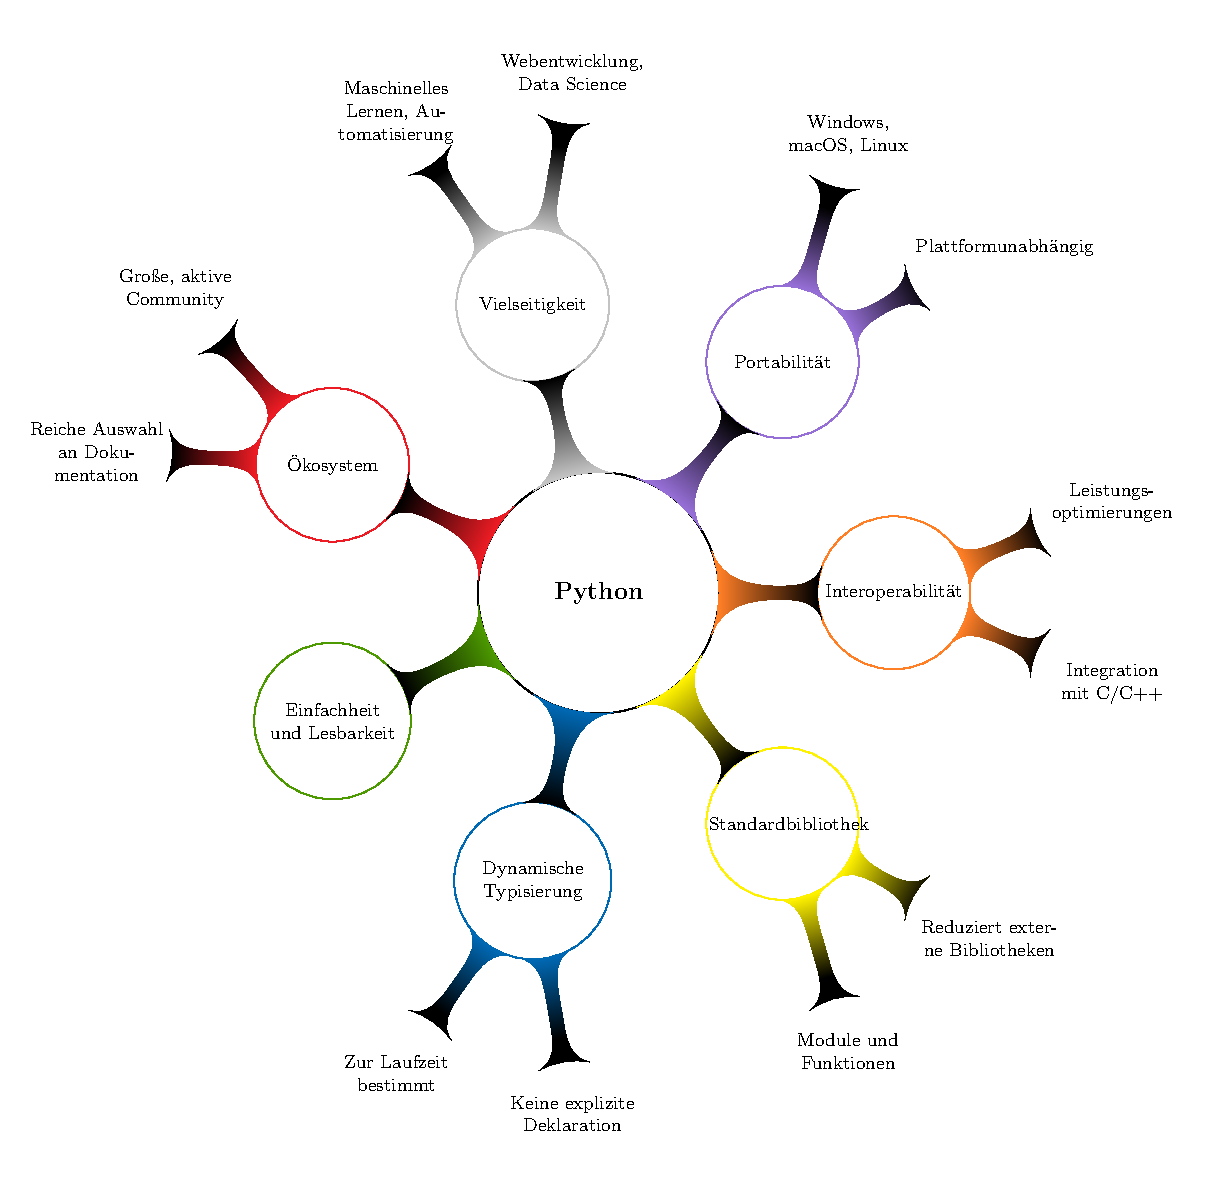
\includegraphics[width=0.6\linewidth,keepaspectratio]{images/Mindmap-Python.pdf}
%\floatnotes{}
%\label{fig:}
\caption{Was ist Python?}
\end{figure}

\subsection{Links}\label{links}

Website \href{https://www.google.com}{Google} und GitHub
\url{https://github.com/ju1-eu} und meine Website
\url{https://bw-ju.de/}

\newpage

\subsection{Quellcode}\label{quellcode}

\begin{lstlisting}[language=C]
/* Quellcode: HalloWelt.c */
#include <stdio.h>

int main() {
   printf("Hallo Welt\n");
   return 0;
}
\end{lstlisting}

\begin{lstlisting}[language={C++}]
// Quellcode: HalloWelt.cpp
#include <iostream>

int main() {
    std::cout << "Hallo Welt" << std::endl;
    return 0;
}
\end{lstlisting}

\begin{lstlisting}
// Markdown
[Google](https://www.google.com)

![Logo 2](images/Logo/Logo2.pdf){width=50%}
\end{lstlisting}

\section{Dokumentenverarbeitung
LaTeX/HTML/Python}\label{dokumentenverarbeitung-latexhtmlpython}

Toolset zur automatisierten Dokumentenverarbeitung mit LaTeX, HTML und
Python.

\subsection{Projektstruktur}\label{projektstruktur}

\begin{itemize}

\item
  \verb|/content|: Vorlagen für Makefile, LaTeX und
  CSS
\item
  \verb|/python-scripte|: Automatisierungsskripte
\item
  \verb|/venv|: Isolierte Python-Umgebung
\end{itemize}

\begin{lstlisting}
# Projektstruktur anzeigen
tree -L 2 --dirsfirst
# Projektstruktur erfolgt nach Python-Projektstandards
# Ausgabe kommentieren
.
├── Mindmap/          # Mindmap-Vorlagen und -Dateien
│   └── Mindmap-Vorlage.tex
├── Tabellen/         # PDF-Tabellen und Inputlisten
│   ├── PDF/
│   └── input-PDFs.txt
├── content/          # Projektvorlagen & -Ressourcen
│   ├── Makefile
│   ├── *.tex        # LaTeX-Vorlagen
│   ├── *.html       # HTML-Vorlagen
│   ├── *.bib        # Literaturverzeichnisse
│   └── *.css        # Stylesheets
├── html/            # HTML-Ausgabedateien
├── images/          # Bilder und Mindmaps
├── md/              # Markdown-Quelldateien
├── python-scripte/  # Automatisierungsskripte
├── tex/             # LaTeX-Ausgabedateien
└── venv/            # Python virtuelle Umgebung
\end{lstlisting}

\subsection{Tools}\label{tools}

\begin{itemize}

\item
  Dokumentenverarbeitung: Markdown, LaTeX, HTML
\item
  Medien: Bild-/PDF-Extraktion, Video-Transkription
\item
  Code-Qualität: pre-commit hooks, Linting
\item
  Versionierung: Git-Integration
\end{itemize}

\begin{lstlisting}[language=bash]
# Python Setup
python3 -m venv venv
source venv/bin/activate
./update_python_packages.sh      # Python-Pakete aktualisieren

# LaTeX
tlmgr install pgf
sudo tlmgr update --all

# Repository initialisieren
git init
# Speichert Git-Zugangsdaten temporär im Speicher, sodass sie nicht bei jedem Push/Pull erneut eingegeben werden müssen.
git config --global credential.helper cache
# GitHub CLI-Tool zur Authentifizierung
gh auth login

# Repository Setup
git remote add origin https://github.com/ju1-eu/notizen_latex_html_python_v1.3.git
git remote add local /Users/jan/notizen_latex_html_python_v1.3.git

# Workflow
git status              # Status prüfen
git add .               # Änderungen stagen
git commit -m "Update"  # Committen
git push origin main    # Nach GitHub pushen
git push backup main    # Lokales Backup

# Branches
git checkout -b feature # Neuen Branch erstellen
git merge feature      # In main mergen
git branch -d feature  # Branch löschen

# Weitere Befehle
git pull               # Updates holen
git log               # Historie anzeigen
git diff               # Änderungen zeigen
git reset --hard HEAD  # Auf letzten Commit zurück


# Pre-commit Setup
pip install pre-commit            # Tool installieren
pre-commit --version             # Version prüfen
# Installation/Update der Hooks
pre-commit clean                 # Cache leeren
pre-commit install              # Hooks installieren
pre-commit autoupdate           # Hooks aktualisieren
pre-commit run --all-files      # Alle Hooks testen
\end{lstlisting}

Konfigurationsdateien:

\begin{lstlisting}
.pre-commit-config.yaml    # Pre-commit Hook-Konfiguration
pyproject.toml            # Python Projekt & Tool-Konfiguration
setup.cfg                # Python Package-Konfiguration
config.yaml             # Skript-Konfiguration
requirements.txt        # Python Abhängigkeiten
requirements-dev.txt    # Entwickler-Abhängigkeiten
\end{lstlisting}

Die wichtigsten Konfigurationen erfolgen in
\verb|.pre-commit-config.yaml| für Hooks und
\verb|config.yaml| für Skript-Optionen.

\subsection{Python Scripte}\label{python-scripte}

\begin{lstlisting}[language=bash]
# Update & Qualitätssicherung
./update_python_packages.sh           # Python-Pakete aktualisieren
./check_pythoncode_quality.sh         # Code-Qualität prüfen (black, isort, flake8, mypy)

# Projekt-Tools
python scriptauswahl.py               # Menü für LaTeX/HTML-Befehle

# Bildverarbeitung
python image_resizer.py               # Bildoptimierung
python create_gallery.py              # Responsive Bildergalerie
python extract_pdf_images.py          # PDF-Bild-Extraktion

# PDF/Video
python pdf_extractor.py               # PDF-Kapitel extrahieren
python youtube_text_extraktor.py      # YouTube-Untertitel/Transkription
\end{lstlisting}

\subsection{Hauptfunktionen}\label{hauptfunktionen}

\begin{itemize}

\item
  LaTeX/HTML-Konvertierung
\item
  Dokumentenformatierung
\item
  Bildverarbeitung
\item
  Git-Integration
\item
  Navigationsaufbau
\end{itemize}

\subsection{Installation}\label{installation}

\begin{lstlisting}[language=bash]
python -m venv venv
source venv/bin/activate
\end{lstlisting}

\subsection{Verwendung}\label{verwendung}

\begin{lstlisting}[language=bash]
python scriptauswahl.py
\end{lstlisting}

\subsection{Voraussetzungen}\label{voraussetzungen}

\begin{itemize}

\item
  Python 3.x
\item
  LaTeX
\item
  Pandoc
\item
  Git
\end{itemize}

\subsection{Lizenz}\label{lizenz}

MIT

\section{Python Package Update
Script}\label{python-package-update-script}

Automatisiertes Update-Tool für Python-Pakete in einer virtuellen
Umgebung.

\subsection{Features}\label{features}

\begin{itemize}

\item
  Update von Produktions- und Entwicklungspaketen
\item
  Backup bestehender Requirements
\item
  Detailliertes Update-Logging
\item
  Fehlerbehandlung
\item
  Farbige Konsolenausgabe
\end{itemize}

\subsection{Voraussetzungen}\label{voraussetzungen-1}

\begin{itemize}

\item
  Python 3.x Installation
\item
  Virtuelle Umgebung (venv)
\item
  requirements.txt / requirements-dev.txt
\item
  Bash/zsh Shell
\end{itemize}

\subsection{Verwendung}\label{verwendung-1}

\begin{lstlisting}[language=bash]
chmod +x update_python_packages.sh
./update_python_packages.sh
\end{lstlisting}

\subsection{Output}\label{output}

\begin{itemize}

\item
  Backup-Dateien (.backup.txt)
\item
  Aktualisierte Requirements
\item
  Update-Log (update\_log.txt)
\end{itemize}

\subsection{Version}\label{version}

2.0 (2024-11-26)

\section{Python Code Quality Check
Script}\label{python-code-quality-check-script}

Automatisierte Code-Qualitätsprüfung für Python-Skripte.

\subsection{Tools}\label{tools-1}

\begin{itemize}

\item
  black (Formatierung)
\item
  isort (Imports)
\item
  flake8 (Style)
\item
  mypy (Typen)
\end{itemize}

\subsection{Verwendung}\label{verwendung-2}

\begin{lstlisting}[language=bash]
chmod +x check_pythoncode_quality.sh
./check_pythoncode_quality.sh
\end{lstlisting}

\subsection{Features}\label{features-1}

\begin{itemize}

\item
  Virtuelle Umgebung Check/Setup
\item
  Tool-Verfügbarkeit Check
\item
  Dateiprüfung
\item
  Farbige Konsolenausgabe
\item
  Fehlerbehandlung
\end{itemize}

\subsection{Voraussetzungen}\label{voraussetzungen-2}

\begin{itemize}

\item
  Python 3.7+
\item
  Virtuelle Umgebung (venv)
\item
  Code-Qualitäts-Tools
\end{itemize}

\subsection{Version}\label{version-1}

1.0 (2024-11-26)

\section{PDF Kapitel Extraktor}\label{pdf-kapitel-extraktor}

Ein Python-Skript zum Extrahieren und Speichern von PDF-Seitenbereichen.

\subsection{Features}\label{features-2}

\begin{itemize}

\item
  Extraktion von Seitenbereichen
\item
  Metadaten-Übertragung
\item
  Optionale Komprimierung
\item
  Fortschrittsanzeige
\item
  Fehlerbehandlung
\end{itemize}

\subsection{Installation}\label{installation-1}

\begin{lstlisting}[language=bash]
python3 -m venv venv
source venv/bin/activate
pip install pypdf2
\end{lstlisting}

\subsection{Verwendung}\label{verwendung-3}

\begin{lstlisting}[language=Python]
# Als Skript
python pdf_extraktor.py

# Als Modul
from pdf_extraktor import extrahiere_kapitel
extrahiere_kapitel("input.pdf", "output.pdf", 1, 5)
\end{lstlisting}

\subsection{Funktionen}\label{funktionen}

\begin{itemize}

\item
  \verb|get\_pdf\_info()|: Liest PDF-Metadaten
\item
  \verb|validiere\_eingaben()|: Prüft
  Benutzereingaben
\item
  \verb|extrahiere\_kapitel()|: Extrahiert
  Seitenbereich
\end{itemize}

\subsection{Version}\label{version-2}

1.0 (2024-11-26)

\section{PDF Bilder Extraktor}\label{pdf-bilder-extraktor}

Python-Tool zur Extraktion von Bildern aus PDF-Dateien.

\subsection{Features}\label{features-3}

\begin{itemize}

\item
  Multi-Format-Extraktion (JPEG, PNG, WebP)
\item
  Qualitätsfilterung
\item
  Bildoptimierung
\item
  Fortschrittsanzeige
\item
  Ausführliches Logging
\end{itemize}

\subsection{Installation}\label{installation-2}

\begin{lstlisting}[language=bash]
pip install PyMuPDF Pillow rich tqdm
\end{lstlisting}

\subsection{Hauptfunktionen}\label{hauptfunktionen-1}

\begin{itemize}

\item
  \verb|PDFImageExtractor|: Hauptklasse für
  Extraktion
\item
  \verb|ImageConfig|: Konfigurationseinstellungen
\item
  Qualitäts- und Größenprüfung
\item
  Bildoptimierung
\item
  Metadatenextraktion
\end{itemize}

\subsection{Verwendung}\label{verwendung-4}

\begin{lstlisting}[language=Python]
config = ImageConfig(
    min_width=200,
    min_height=200,
    max_size_mb=10.0,
    quality=90,
    optimize=True
)

extractor = PDFImageExtractor(
    pdf_path="input.pdf",
    output_dir="images",
    project_name="project",
    image_format="png",
    config=config
)

stats = extractor.extract_images()
\end{lstlisting}

\subsection{Version}\label{version-3}

1.0 (2024-11-26)

\section{HTML Galerie Generator}\label{html-galerie-generator}

Python-Tool zur Erstellung responsiver Bildergalerien.

\subsection{Features}\label{features-4}

\begin{itemize}

\item
  Grid-Layout \& Lightbox
\item
  Theme-Optionen
\item
  Bildoptimierung
\item
  Thumbnails
\item
  Sortierung/Filter
\item
  Lazy Loading
\end{itemize}

\subsection{Installation}\label{installation-3}

\begin{lstlisting}[language=bash]
pip install pillow
\end{lstlisting}

\subsection{Hauptkomponenten}\label{hauptkomponenten}

\begin{itemize}

\item
  \verb|GalleryConfig|: Galerie-Einstellungen
\item
  \verb|GalleryGenerator|: Galerie-Generierung
\item
  Theme-Generator
\item
  Thumbnail-Erstellung
\item
  Responsive Design
\end{itemize}

\subsection{Verwendung}\label{verwendung-5}

\begin{lstlisting}[language=Python]
config = GalleryConfig(
    title="Meine Galerie",
    theme="light",
    columns_desktop=4,
    thumbnail_size=(300, 300)
)

generator = GalleryGenerator(
    image_dir="images",
    project_name="project",
    output_dir="gallery",
    config=config
)

generator.generate_gallery()
\end{lstlisting}

\subsection{Version}\label{version-4}

1.0 (2024-11-26)

\section{YouTube Text Extraktor}\label{youtube-text-extraktor}

Tool zur Extraktion von Text aus YouTube-Videos.

\subsection{Features}\label{features-5}

\begin{itemize}

\item
  Untertitel-Extraktion
\item
  Audio-Download
\item
  Whisper-Transkription
\item
  Automatische Formatbereinigung
\item
  Mehrsprachig (DE/EN)
\end{itemize}

\subsection{Installation}\label{installation-4}

\begin{lstlisting}[language=bash]
pip install youtube-transcript-api pytube whisper
\end{lstlisting}

\subsection{Funktionen}\label{funktionen-1}

\begin{lstlisting}[language=Python]
prüfe_url(url: str) -> bool
hole_video_id(url: str) -> str
hole_untertitel(video_id: str) -> str|None
extrahiere_audio(url: str) -> str|None
transkribiere_audio(audio_pfad: str) -> str|None
extrahiere_text_aus_video(url: str) -> str
speichere_text(text: str) -> None
\end{lstlisting}

\subsection{Verwendung}\label{verwendung-6}

\begin{lstlisting}[language=Python]
from youtube_text_extraktor import extrahiere_text_aus_video

url = "http://youtu.be/VIDEO_ID"
text = extrahiere_text_aus_video(url)
\end{lstlisting}

\subsection{Version}\label{version-5}

1.0 (2024-11-26)

%% Anhang
%\clearpage
%\appendix

\clearpage
\printbibliography
\end{document}
